
%%%%%%%%  Document class  %%%%%%%%%%%%
\documentclass[11pt, letterpaper, fleqn]{article}
% fleqn is for left aligned equations

%%%%%%%%  Packages   %%%%%%%%%%%%%%%%
\usepackage{amsmath,amssymb}
\usepackage[english]{babel}
\usepackage{graphicx} 
\usepackage{indentfirst}
\usepackage{times}
\usepackage{array}
\usepackage{setspace}
\usepackage[backend=bibtex,style=authoryear]{biblatex}
\usepackage{filecontents}
\bibliography{library.bib,other.bib}
\usepackage{tocloft}
\usepackage{tocbibind}
\usepackage{xpatch}
\usepackage{float}
\usepackage{wrapfig}
\floatstyle{plain} 
\renewcommand{\floatpagefraction}{.8}
\restylefloat{figure}
\newcommand{\listappendicesname}{}
\newlistof{appendices}{apc}{\listappendicesname}
\newcommand{\appendices}[1]{\addcontentsline{apc}{appendices}{#1}}
\newcommand{\newappendix}[1]{\section*{#1}\appendices{#1}}

\newcommand{\listequationsname}{List of Equations}
\newlistof{myequations}{equ}{\listequationsname}
\newcommand{\myequations}[1]{%
\addcontentsline{equ}{myequations}{\protect\numberline{\theequation}#1}\par}

\parindent0mm
\setlength{\parindent}{4em}
\setlength{\parskip}{1em}
\setkeys{Gin}{width=0.9\textwidth}

%%%%%%%%  Page Setup %%%%%%%%%%%%%%%%%%
\usepackage[margin= 2cm]{geometry}

% !Rnw root=Thesis_doc.RNW

%%%%%%%% Document %%%%%%%%%%%%%%%%%%%
\usepackage{Sweave}
\begin{document}
\Sconcordance{concordance:Thesis_doc.tex:Thesis_doc.Rnw:%
7 225 1 1 6 1 2 6 1 1 15 15 1 1 33 5 0 1 2 10 1 1 41 9 1 1 15 23 1 1 26 %
1 3 171 1}

\Sconcordance{concordance:Thesis_doc.tex:Thesis_doc.Rnw:%
7 225 1 1 6 1 2 6 1 1 15 15 1 1 33 5 0 1 2 10 1 1 41 9 1 1 15 23 1 1 26 %
1 3 171 1}

\pagenumbering{roman}
\thispagestyle{empty}

\vspace*{1\baselineskip}
\begin{center}

\text{PREDICTING THE GROWTH RESPONSE OF SMALL PONDEROSA PINE TREES UNDER} 
\text{VARYING LEVELS OF OVERSTORY RETENTION, VEGETATIVE COMPETITION AND}
\text{SITE QUALITY} 

\text{By}

\text{Colin Patrick Kirkmire} 

\text{B.Sc. Forest Management, University of Washington, Seattle, Washington, 2015} 

\text{Thesis} 

\text{presented in partial fulfillment of the requirements
for the degree of} 

\text{Master of Science}\\
\text{in Forestry} 

\text{The University of Montana}\\
\text{Missoula, MT} 

\text{July 2017} 

\text{Approved by:}\\ 
\vspace{10 mm}
\text{Scott Whittenburg, Dean of the Graduate School}\\
\text{Graduate School} 
\vspace{10 mm}

\text{Dr. David L.R. Affleck, Co-Chair}\\ 
\text{Forest Management} 
\vspace{10 mm}

\text{Dr. John Goodburn, Co-Chair}\\ 
\text{Forest Management} 
\vspace{10 mm}

\text{Dr. David Patterson}\\ 
\text{Statistics} 
\vspace{10 mm}

\text{Dr. Peter Kolb}\\ 
\text{Forestry Extension} 
\end{center}


\newpage
\thispagestyle{empty}
\vspace*{5\baselineskip}
\begin{center}
\textbf{\large{Predicting the Growth Response of Small Ponderosa Pine Trees under Varying levels of Overstory Retention, Vegetative Competition and Site Quality}} \\[1pt] 
\vspace*{5\baselineskip}
\text{Colin Kirkmire} \\[1pt]
\vspace*{3\baselineskip}
\text{A thesis submitted to the Graduate Faculty of }\\[1pt]
\text{the University of Montana}\\[1pt]
\text{in partial fullfillment of the}\\[1pt]
\text{requirements for the degree of}\\[1pt]
\text{Master of Science}\\[1pt]
\vspace*{3\baselineskip}
\text{Department of Forest Management}\\[1pt]
\text{College of Forestry and Conservation}\\[1pt]
\text{University of Montana}\\[1pt]
\vspace*{3\baselineskip}
\text{Missoula, Montana}\\[1pt]
\vspace*{1\baselineskip}
\text{{2016}} \\[1pt]
\vspace*{7\baselineskip}
\text{Advised by Dr. David L.R. Affleck and Dr. John Goodburn}\\[1pt]
\vspace*{7\baselineskip}
\end{center}

\newpage
\large 
\begin{center}
\textbf{DEDICATION}\\[1pt]
\end{center}

\newpage
\large 
\begin{center}
\textbf{BIOGRAPHY}\\[1pt]
\end{center}
\normalsize

\newpage
\large 
\begin{center}
\textbf{ACKNOWLEDGEMENTS}\\[1pt]
\end{center}
\normalsize

I would first like to extend appreciation to the INGY Cooperators, particularly those who participated in the Small Tree Competing Vegetation Study (STCV) for their commitment to this long term study. Their participation required that many stands not be harvested for the duration of the study and a substantial monitary cost over 15 years.

I also owe a debt of gratitude to the many INGY technicians and researchers who have worked on the STCV before me. The completion of the dataset would not have been possible without your ``boots on the ground'' and careful acquisition of measurements.

Thank you to my advisors Dr. David Affleck and Dr. John Goodburn for giving me the opportunity to choose a challenging research topic and for support as I developed the skills to accomplish this research.

I thank my family for their support and excusing my absense while pursuing this research.  I would also like to thank all of the previous generations of my family that have enjoyed careers in forestry in the Western United States.  Your life-long passion for our forests and the communities they support is something that constantly motivates me.

To my friends in forestry, I thank you for both your commeraderie and friendly competition. I hope that we may never stop developing and sharing our knowledge of forest management. 






\newpage
\large 
\begin{center}
\textbf{TABLE OF CONTENTS}\\[1pt]
\end{center}

\normalsize
\tableofcontents
\large 
\begin{center}
\textbf{LIST OF APPENDICES}\\[1pt]
\end{center}
\listofappendices

\newpage
\large 
\begin{center}
\textbf{TABLES}\\[1pt]
\end{center}
\normalsize
\listoftables
\normalsize

\newpage
\large 
\begin{center}
\textbf{FIGURES}\\[1pt]
\end{center}
\normalsize
\listoffigures

% !Rnw root=Thesis_doc.RNW

\newpage
\pagenumbering{arabic}
\setcounter{page}{1}
\large 
\begin{center}
\textbf{Introduction}\\[1pt]
\end{center}
\normalsize
\noindent 
\text{This will be the introduction}
\textbf{Objectives}\\[1pt]
\textbf{Ecology of Ponderosa Pine Regeneration}\\[1pt]


Many studies have found that understory vegetation competition slows the early development of ponderosa pine  

Busse et al. found that the presence of understory vegetation adversely affected the growth of ponderosa pine for an estimated 20 years which is a relatively short time in a long stand rotation (\cite{Busse1996}). However, the authors also noted that there is a long term benefit to the upper soil horizon from maintaining understory vegetation in the form of greater C and N.

Composition of forest understory species are controlled by overstory trees which filter light, moderate understory air and soil temperature,and directly compete for soil water and nutrients cite(need Spurr and Barnes 1980). Conifer reforestation efforts are often hampered by the aggressive and competitive ability of \emph{Carex} and \emph{Calamagrostis} because they respond positively to the removal of the overstory (Sloan and Ryker 1986). 





\begin{figure}[ht]
\begin{center}
    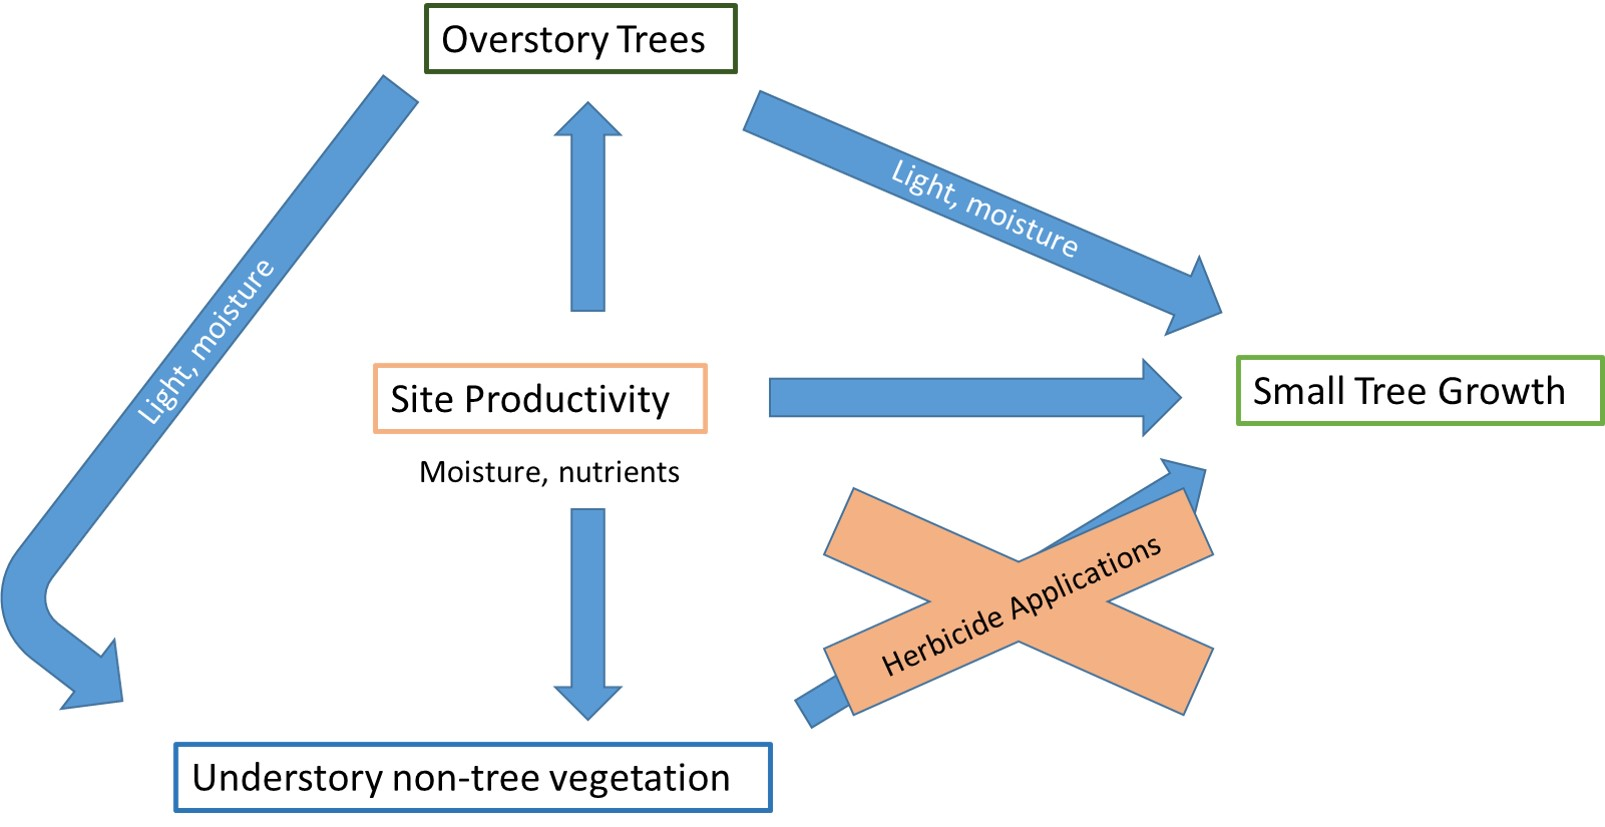
\includegraphics[width=160mm]{comp_flowchart.jpg}
    \caption{Biological framework of small tree growth. Small trees are defined as those that have a DBH less than 3.5 in}
    \label{fig:chart}
\end{center}
\end{figure}

\begin{figure}[ht]
\begin{center}
    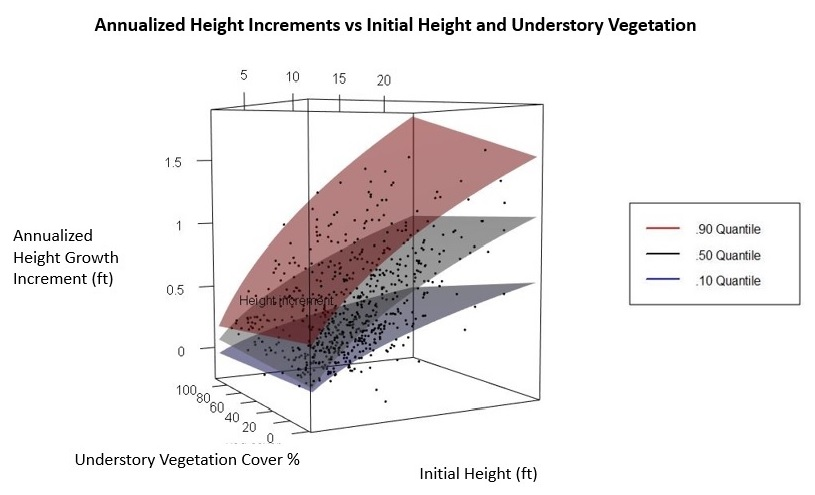
\includegraphics[width=160mm]{threedveg.jpg}
    \caption{Quantile Regression Visualization}
    \label{fig:Quantregvis}
\end{center}
\end{figure}

\begin{figure}[ht]
\begin{center}
    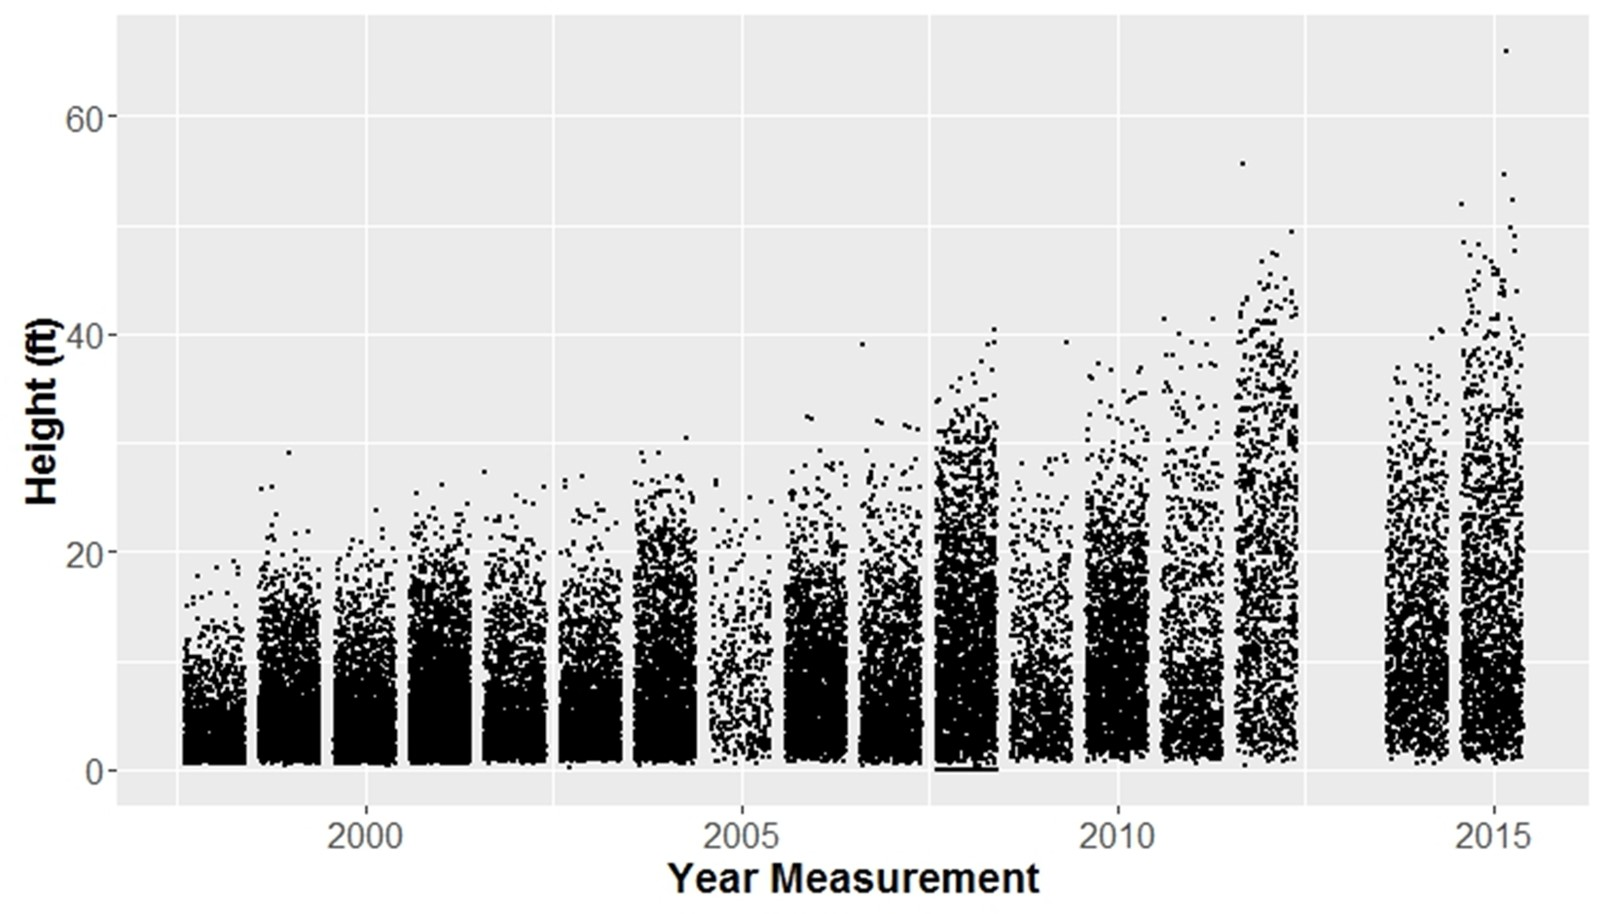
\includegraphics[width=160mm]{all_trees.jpg}
    \caption{Total height of all tagged small trees over the course of the study}
    \label{fig:alltrees}
\end{center}
\end{figure}





\begin{figure}
\begin{center}
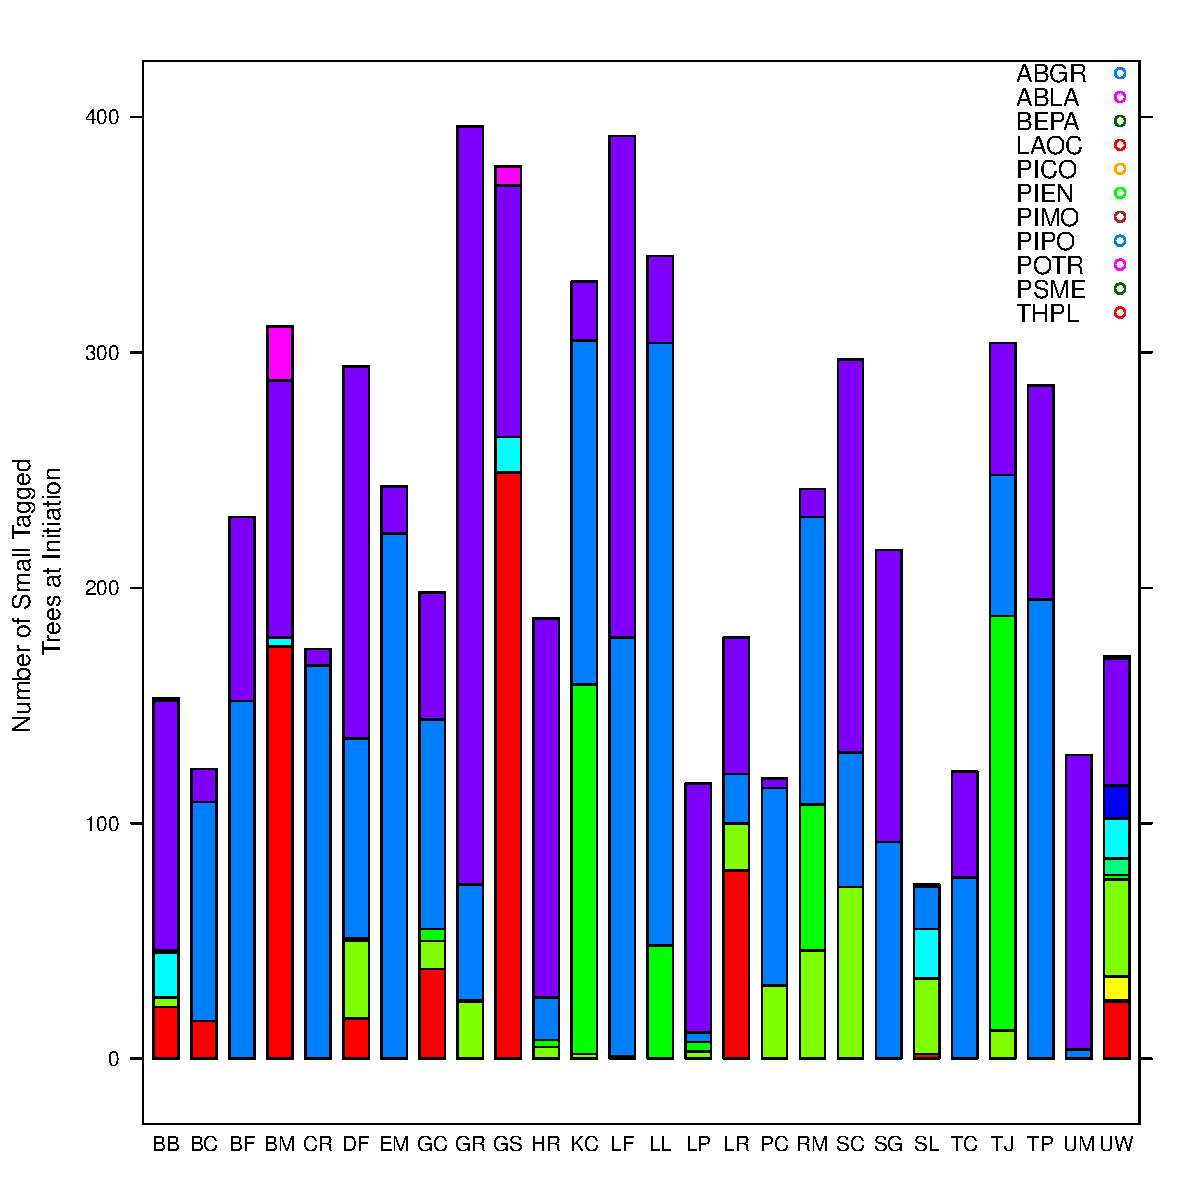
\includegraphics{Thesis_doc-speccomp}
\end{center}
\caption{Species Composition of Small Tagged Trees in Installations with more than 60 Ponderosa Pine}
\end{figure}



% !Rnw root=Thesis_doc.RNW


\newpage
\clearpage
\begin{center}
\section{Methods}
\end{center}
\normalsize
\subsection{Sampling Strategy}
\doublespacing
Twenty-nine study sites (termed ``installations'') were established on a variety of cooperative member ownership ranging from the eastern slopes of the Cascade Mountains to western Montana. The installations fall within three distinct geographic areas; central Washington, eastern Washington/Idaho and western Montana. \\[4pt]


\begin{Schunk}
\begin{Soutput}
pdf 
  2 
\end{Soutput}
\end{Schunk}

\begin{figure}[ht]
\begin{center}
    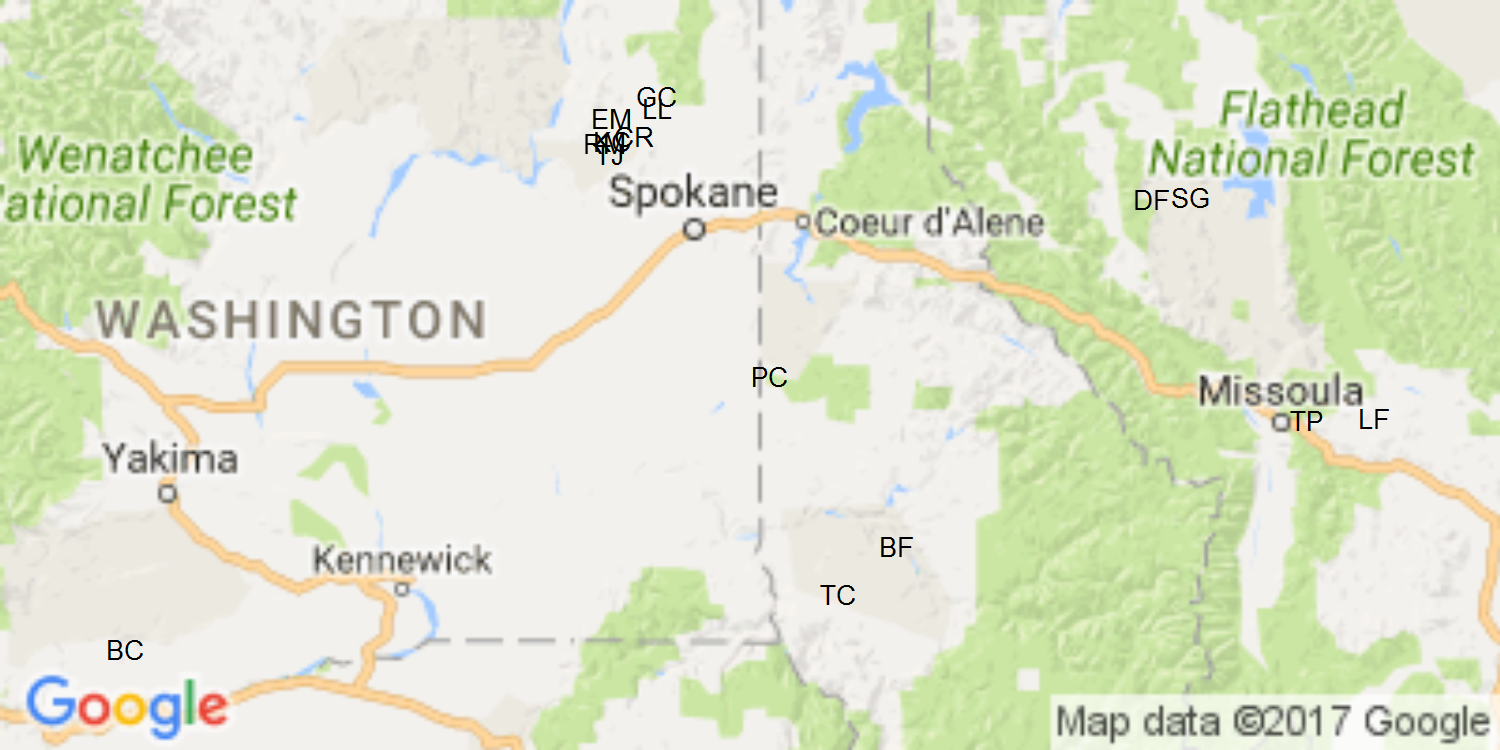
\includegraphics[width=.8\textwidth]{inst_map.png}
    \caption{Map of STCV Installations}
    \label{fig:map}
\end{center}
\end{figure}


\begin{figure}
\begin{center}
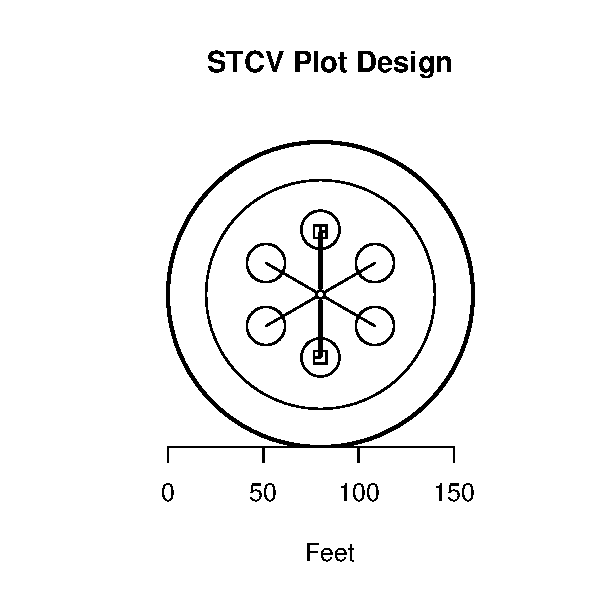
\includegraphics{Thesis_doc-sampleplot}
\end{center}
\caption{Design of STCV Sampling Plot. Note that transect points and quadrants exist for all six small tree plots although only illustrated on two.}
\end{figure}


\begin{figure}
\begin{center}
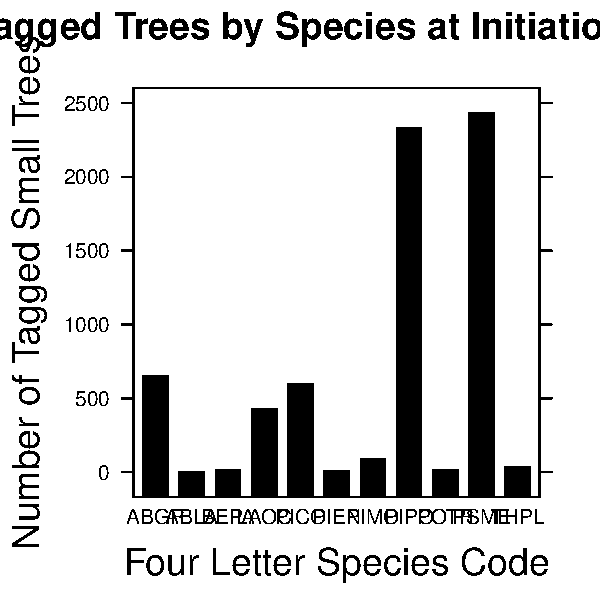
\includegraphics{Thesis_doc-species}
\end{center}
\caption{Number of Small Tagged Trees by Species}
\end{figure}


Installations were established in stands with various forest cover (e.g., mixed ponderosa pine, Douglas-fir, and grand fir types), with each stand exhibiting relatively homogeneous levels of site quality, overstory tree density, and understory competition.  Installations were located in recently harvested stands that were either clearcut or harvested with one of the aforementioned variable retention harvest systems: shelterwood, seed tree and heavy thinning. \\[2pt]


The site productivity of the installations was measured according to the dominate site tree which varied between ponderosa pine, douglas fir and ... Selecting only stands with greater than 60 small tagged ponderosa for this analysis effectively removed nearly all stands that measured site index with a species besides ponderosa pine.

There appears to be a group of six installations with similarly low overstory retention levels and high site index values.  This makes sense from a forest management perspective, that relatively little residual overstory would be left on sites with higher productivity.  These installations could be used to develop the understory model since they are so similar in overstory and site productivity. There are many other installations that can be brought in later to expand the model to other various levels of productivity and overstory retention.

The temporal initiation of installations varied with most being established in the last years of the 1990s and early 2000s.  Three check plots were also installed to audit the quality of the data collection efforts. Treatments were randomly assigned to seven plots within each installation (Figure 3).  Three plots received multiple applications of regionally effective herbicide.  The remaining four plots are split between the one-time treatment group (just one application of herbicide) and control plots which received no herbicide treatment.\\[2pt]

The primary objective of the different herbicide treatments is to decouple the direct and indirect effects of removing overstory. The removal of the overstory increases available light which is hypothesized to encourage small tree growth as well as non-tree vegetation.  The herbicide treatments allow us to see how small trees grow under reduced overstory without the presence of a corresponding increase in non-tree vegetation.\\[2pt]

Figure 3 shows the temporal scope of the data collection as well as herbicide applications and overstory measurements. An attempt to capture growth at each installation at four year intervals was successful for many installations but in some cases the intervals are somewhat irregular (i.e., 3-5 years in length). The schedule of measurements was based on the twelve-year projection cycles that were used by participating cooperative members.\\[2pt]
\begin{figure}
\begin{center}

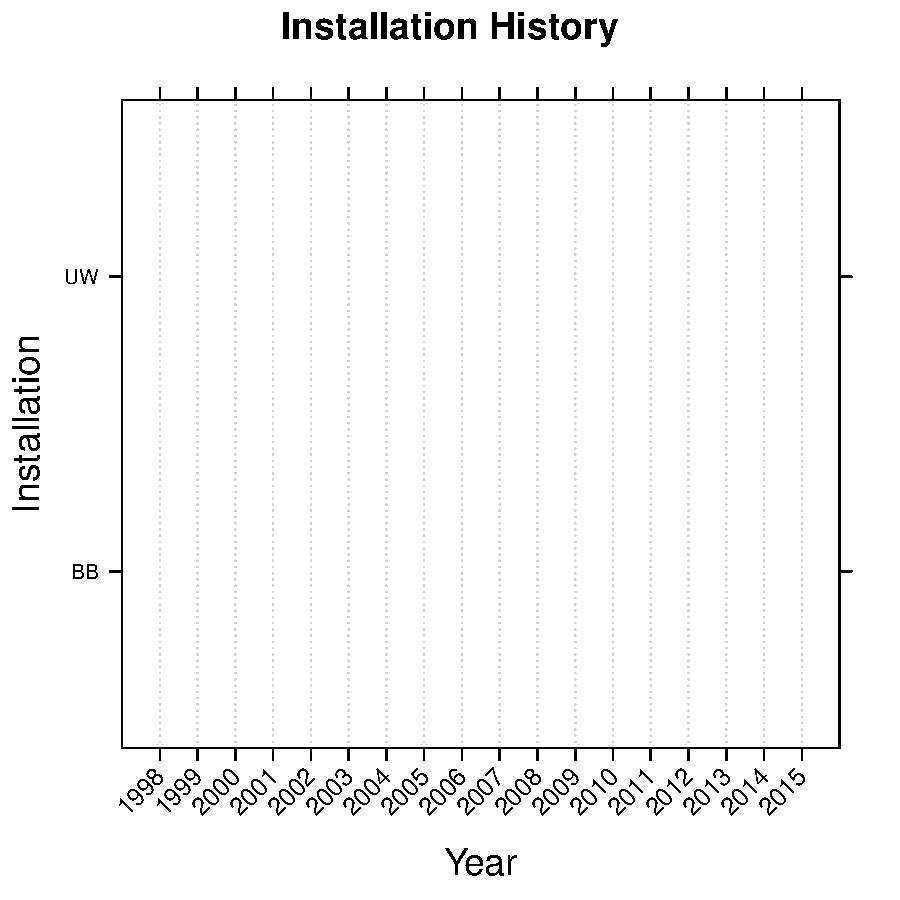
\includegraphics{Thesis_doc-timeline}
\end{center}
\caption{Timeline of Installation Measurements and Treatments}
\end{figure}



A point of concern is that some measurements were taken at times that would not have allowed for the herbicide applications to take full effect. That is, several measurements were concurrent with or followed too quickly after the first herbicide application.  This necessitated careful selection of the appropriate measurement years on a per installation basis. Generally, "first interval years" were selected such that one to three years following the initial herbicide application were included to allow for the herbicide to take effect. Ultimately, the growth measurements will be put on the same temporal scale of periodic annual increment regardless of whether they were collected on a 3, 4 or 5-year interval. \\[2pt]


When comparing the vegetation volumes between the control and the herbicide plots at the beginning of the measurement intervals, it is apparent that there is a large drop in volume within installations with large amounts of understory vegetation when herbicide is applied. However, the herbicide applications failed to contribute to a marked difference in volume in installations of little volume in control plots.

Each plot contains a series of nested plots that decrease in area with physiologically smaller vegetation units (Figure 4). Starting with the full extent of the plot, overstory trees (> 10.5 in DBH) were measured on an approximately half acre. Medium trees, with DBH greater than 3.5 in but less than 10.5 in were measured on a smaller nested plot of roughly a quarter acre.
Small trees were measured on six .007 acre plots 60 degrees apart from plot center at a distance of approximately 30 feet.  Small trees are defined as those that have a DBH less than 3.5 in yet are greater than .5 ft in height for shade tolerant species or 1 ft for shade intolerant at the time of initial measurements.\\[2pt]

There were two sampling methods used to measure vegetative competition. The first was transect based where point measurements of vegetation were obtained at one foot intervals along a 40 ft transect.  We also took vegetation measurements in the middle of the small tree plots in the form of both 1m2 and 4m2 grids. These vegetation measurements quantified separately the amounts of forbs, grasses and shrubs to the species level.  This is an example of how the resolution of the data goes beyond the scope of this analysis though will undoubtedly be of use in future research efforts.\\[2pt]

\subsection{Statistical Approach}

This research seeks to address the question of how to predict the response distribution of small Ponderosa Pine tree height growth increments.  To achieve this ends, a nonparametric statistical regression technique known as quantile regression will be utilized to fit growth curves over select quantiles of the response distribution heights by a set of ecologically and statistically significant predictors. Thus we will be able to predict the heights of the "fastest", "median" and "slowest" growing trees.
This research has widespread applications in the management of Ponderosa Pine stands since the fastest growing trees are
presumably those that progress into the canopy and those that may be retained with preference in the context of a thinning.\\[2pt]

The model is predictive in the sense that it will attempt to predict several quantiles height growth increments. For example, the model will not be able to determine whether specific trees will be projected to be above or below the .9 quantile line but rather predict what the .9 quantile height itself is for a given set of predictors. If enough information was known about these trees to predict which would be the fastest growing trees, it would negate the utility of quantile regression.\\[2pt]

The fact that quantile regression attempts to characterize the entire distribution of heights makes it much more difficult to test and validate than an ordinary least squares regression.  The regression estimates at the selected quantile provide predictions for that specific quantile and it is likely that the predictive ability of the model changes at different quantiles.  For example, the model may predict the median better than the upper quantile. \\[2pt]

To evaluate the model, three quantiles will be fitted to represent the range of the response distribution (.90,.50 and .10).  The height increments from the withheld plot data will then be compared to the height of the predicted quantile regression line for its corresponding predictor variables.  For example, if the .90 quantile plane is a good fit, then theoretically 10\% of the height increments will lie above the plane and 90\% below.  The .50 and .10 planes will be evaluated in a similar manner. \\[2pt]

	If it appears that there is some commonality between the tree height increments that are falling below/above the quantile plane...\\[2pt]

Following this evaluation, a random sample of tagged subject trees will be selected to have their height growth increments predicted in the USFS Forest Vegetation Simulator (FVS).  These predicted height increments will then be evaluated as above.  It is not expected that .90 of the predicted tree heights will fall below that .90 quantiles for example. The FVS small tree growth sub-model is based on a least squares regression equation so it is very unlikely that the predicted heights will correspond to the quantile planes.   Rather, this exercise is to illuminate how far from the actual growth response distribution of FVS predictions can be.\\[2pt]

\newpage
\subsection{Variable Acquisition}

\textbf{Understory Tree:}
The tallies of small trees from each small tree plot (STP) were summed by height class and then multiplied by 138.73 to obtain per acre estimates.  The number of trees greater than the subject trees was found by summing all height class tallies with class midpoints greater than the height of the subject tree. Crown length was found by subtracting the crown base from the total height.  Crown width was found as an average of the two perpendicular measurements of crown width obtained in the field. Basal diameter and DBH required no further refinement.

\textbf{Understory Vegetation:}

Only the 1m vegetation plots were utilized in this study since they were used for the duration of the study.  Average differences at the STP level between base and top height measurements were found separately for forbs,low shrubs, high shrubs and grasses.  Ocular estimates of percentage cover were found for polyvegetation, forbs, low shrubs, high shrubs and grasses.  Average height differences for low shrubs, high shrubs, forbs were calculated for the 30 transect points corresponding to each small tree plot.  Percentage cover of grass obtained ocularly through a 6in by 6in grid and top height of grasses were also averaged over the length of the transect.

\textbf{Overstory Vegetation:}

Dead overstory tree records were removed from the analysis.  Basal area was calculated for each overstory tree was aggregated from both the .26ac and .46ac overstory plots to provide a per acre estimate of basal area. Zero basal area per acre (BAPA) were assigned to installations without an overstory record due to clearcut. Basal area per acre was linearly interpolated between measurement years to provide estimates for years of small tree and understory measurement.  The initial and final years of overstory measurent provided limits of the interpolation meaning that a vegetation measurement year preceding or following the overstory measurements would be assigned the BAPA calculated for the initial or final Overstory measurement year, respectively.
Crown competition factor (CCF) was obtained by calculating crown width as an average between the two perpendicular measurements of width and then converting crown width to crown area in square feet. Crown area was then computed in terms of percent of an acre (taking into account the plot size that each overstory tree was sampled in). Linearily interpolated estimates of plot level CCF were obtained in the manner described previously for BAPA.
Trees per acre (TPA) is calculated from the plot level aggregation of the two overstory tree plots.

\textbf{Site Quality:}
Slope, elevation and aspect were calculated using Google Earth Engine (\cite{googleearthengine}) for each plot's coordinates. Slope is in units percentage and elevation in meters. Aspect was transformed by taking $\cos$((aspect*$\pi$)/180).


Site index was included from STCV records of each installation's initiation. Site index species was Ponderosa Pine for the installations included in analysis although many other species were used at other installations.




\newpage
\subsection{Variable Selection}


\par Only the installations with greater than 60 ponderosa pine tagged small trees at initiation will be included in the model.  Within these installations, the 6th small tree plots will be withheld as validation data. The check plots and installations that have sustained a post-initiation harvest are also excluded from analysis.  

The objective is to obtain a parsimonious model that is easily understood and informed by our understanding of the factors surrounding small tree growth. The variable selection process for each individual quantile will be guided by the ecological framework behind small tree growth.  The predictor variables will be selected from the four previously mentioned categories of ecological factors that affect tree growth (see Figure \ref{fig:chart} on page \pageref{fig:chart}). These categories are overstory measures, understory non-tree vegetation, site productivity and other small tree measures.  The square root of initial height (height at the beginning of measurement period) explains much of the variability in height growth increment and will be included as a predictor in the base model.


The order of variable selection categories will proceed in the following order; understory tree, understory non-tree vegetation, overstory and finally site productivity. The first two variables; understory non-tree, and understory small tree will be selected from the control plots of a group of installations of comparable site and overstory conditions. Once an ``understory model'' is established, the selection of overstory and site variables will proceed in that order.  These two final categories necessitate the ``linking''of all selected ponderosa pine installations. 



To evaluate the utility of higher-order polynomial expressions of predictor variables, generalized additive models (GAM) with  smoothers of first-order predictors will be used. If inclusion of a higher-order predictor is justified by the partial residual lot from a GAM then it will be considered alongside all other predictors and as an interaction term.

Variable selection from within these categories will be made with respect to their importance in descrbing trends in the median ($\tau$=.5). Within each category of ecological factor, a subset of relevant variables will be considered that includes two-way interactions between the previously selected variables and the category under evaluation. This subset of variables will also take into consideration the practicality of the predictors.

The \texttt{quantreg} package by Roger Koenker cite(Koenker) will be used to fit quantile regression surfaces individually for the specified quantiles (specified as $\tau$ values: .90, .50, .10).  This allows for differences in the selected predictor variables between the quantile planes.
Model building will proceed from category to category with the model of lowest AIC being selected as the model carried forward to the next category. 


Selecting a single dimension from each ecological category of small tree competition also has practical advantages.  If a land manager desired to reproduce a similar set of quantile curves for another ecological system or wanted to compare small tree growth to that of the curves produced in this effort, they would need only to collect a singular measure of competition from each of these categories rather than the extensive measurements that the STCV study has undertaken.




% !Rnw root=Thesis_doc.RNW


\newpage
\subsection{Variable Selection Results and Model Evaluation}

\begin{table}[h]
\small
\caption{Akaike Information Criterion (AIC) for .5 Quantile Regression by Category of Small Tree Competition  }
\begin{center}
\begin{tabular}{cccccccccc}
\hline\hline
{Small Tree}&{n}&{AIC}&
{Vegetation}&{n}&{AIC}&
{Overstory}&{n}&{AIC}&
\\


\hline
Nothing&$1816$&$3083.98$&POLV.cov&4228&4953.03&BAPA&4228&4539.63\tabularnewline
SmallTPA&$1816$&$2843.32$&F.cov&4228&5001.07&CCF&4228&4363.87\tabularnewline
Two&$1811$&$3075.37$&LS.cov&4228&5009&\textbf{TPA}&4228&4272.83\tabularnewline
Four&$1811$&$3065.19$&HS.cov&4228&4999.4&&&\tabularnewline
Six&$1811$&$2990.19$&G.cov&4228&5005.13&Site&n&AIC\tabularnewline
Eight&$1811$&$2944.22$&\textbf{F.diff}&4228&4783.02&Slope&4228&4218.55\tabularnewline
Ten&$1811$&$2929.06$&LS.diff&4228&4924.31&\textbf{SI}&4228&4018.82\tabularnewline
Twelve&$1811$&$2909.83$&HS.diff&4228&4861.02&Elevation&4228&4273.61\tabularnewline
Fourteen&$1811$&$2948.04$&G.diff&4228&4910.01&Aspect&4228&4190\tabularnewline
Fifteen&$1811$&$2965.70$&F.tran&4228&4958.23&&&\tabularnewline
TGT&$1811$&$2896.52$&LS.tran&4228&4973.72&&&\tabularnewline
BD&$1814$&$2359.86$&HS.tran&4228&4929.58&&&\tabularnewline
DBH&$1334$&$2053.96$&G.tran.diff&4228&4893.88&&&\tabularnewline
CrownWidth&$1813$&$2802.97$&G.tran.cov&4226&5008.45&&&\tabularnewline
\textbf{CrownLength}&$1808$&$2705.84$&&&&&&\tabularnewline



\hline
\end{tabular}
\end{center}
\label{tab:dum1}
\end{table}


\newpage

\begin{figure}
\begin{center}
\begin{Schunk}
\begin{Sinput}
> sr.ht.gam<-gam(annual.gr4$ht_annual~s(annual.gr4$srHeight_Total))
> plot(sr.ht.gam,residuals=T,se=T,pch=".")
> cl.ht.gam<-gam(annual.gr4$ht_annual~annual.gr4$srHeight_Total+s(annual.gr4$CrownLength))
> plot(cl.ht.gam,residuals=T,se=T,pch=".")
\end{Sinput}
\end{Schunk}
\end{center}
\caption{Timeline of Installation Measurements and Treatments}
\end{figure}



% !Rnw root=Thesis_doc.RNW


\newpage
\newappendix{Bibliography} 
\printbibliography
All analyses were performed using the R statistical software
R version 3.3.0 (2016-05-03). This thesis was compiled using the document preparation software \LaTeX.


\newpage
\begin{singlespace}
\newappendix{Variable Selection Steps}
\begin{enumerate}
\begin{small}
  \item{Select intallations with >60 \emph{P. Ponderosa} small tagged trees at initiation}
  
  \item{Select installations of similar overstory basal area and site productivity}
  
  \item{Retain the sixth small tree plot of each installation for validation}
  
\item{Create a list of the practical predictor variables within each category:
  \begin{itemize}
         \item {Understory Tree (UT)}
         \item {Understory Non-tree (UV)}
         \item {Overstory Tree (OT)}
         \item {Site Productivity (SP)}
 \end{itemize}
}
  
  \item{For each candidate variable in UT generate a generalized additive model (GAM) using the base model and only the control plots (no herbicide):
  \begin{center}
\begin{equation}\label{eq:Eq1}
  \Delta \textrm{ height annual}=\sqrt{\textrm{ initial height }}+\textrm{ candidate small tree variable}
\end{equation}
  \end{center}
  }
  
  \item{Visually examine the results and the partial residual plots of the models produced in 5}
  
  \item{Include quadratic terms of variables in the list of candidate variables if warranted}
  
  \item{Fit a quantile regression model with each candidate variable for$\textrm{ $\tau$}=.5$ using the quantreg package
    \begin{center}
\begin{equation}\label{eq:Eq2}
  \emph{Q}_{.50}\Delta \textrm{ height annual}=\sqrt{\textrm{ initial height }}+\textrm{ candidate small tree variable}
\end{equation}
  \end{center}
  }
  
  
  \item{Calculate the AIC for each model within the UT category}
  
  \item{Select the variable from the model with the lowest AIC to be carried forward into UV category}
  
  \item{Repeat steps 5-10 for the UV variables}
  \item{Select variables from the overstory and site productivity categories using the process outlined in steps 5-11 using all installations selected in step 1 (and all plots)}
  \item{Using the variables selected for the $\tau$=.5, fit quantile regressions for $\tau$=.1,.9. This will estimate different b_${\tau}$ for each specified quantile.\\
  
  \textbf{Final Models:}\\

\begin{center}
\begin{equation}\label{eq:Eq3}
 \Delta _{\tau} =\textrm{b}_{0,\tau}\sqrt{\textrm{h}}+\textrm{b}_{UT,\tau}\textrm{UT} 
 + \textrm{b}_{UV,\tau}\textrm{UV}+\textrm{b}_{OT,\tau}\textrm{OT}+\textrm{b}_{SP,\tau}\textrm{SP}
  \end{equation}
  \end{center}
\end{small}
\end{enumerate}
\end{singlespace}


\newpage
\newappendix{Equations}
\listofmyequations







\end{document}
